%%%%%%%%%%%%%%%%%%%%%%%%%%%%%%%%%%%%%%%%%
% BAKALÁŘSKÁ PRÁCE			%
% JAKUB FLAŠKA				%
% Šablona převzata ze stránek KSE	%
% (C) FJFI ČVUT v Praze			%
%%%%%%%%%%%%%%%%%%%%%%%%%%%%%%%%%%%%%%%%%

% Typ dokumentu
\documentclass[a4paper,12pt]{report}	% report - jednostranný tisk

%%%%%%%%%%%%%%%%%%%%%%%%%%%%%%%%%%%%%%%%%%%%%%%%%%%
%% Pouzite balíčky

% Kódování a zpracování ČJ
%\usepackage[czech]{babel}	% cestina
\usepackage[T1]{fontenc}	% balicek fontu
\usepackage[utf8]{inputenc}	% cestina
% Vytvoření indexu a seznamu použité literatury
\usepackage{index}		% vytvoření obsahu
\usepackage[pdftex]{hyperref}	% vygeneruje rejstřík při použití pdflatex
\usepackage{cite}		% vytvoření literatury
\usepackage{multibib}		% více zdrojů literatury
% Práce s obrázky
\usepackage{graphicx}		% obrázky
\usepackage{subfig}		% více obrázků v políčku
% Ostatní
\usepackage{listings}		% vkladani zdrojoveho kodu
\usepackage[usenames]{color}	% použití barevného textu
\usepackage{url}		% zpracování www adresy
\usepackage{verbatim}		% moznost viceradkovych kommentaru prikazem \begin{comment}
\usepackage{array}		%
\usepackage{caption}		% Popisky obrázků jiným písmem, než zbytek textu.
\usepackage{amsmath}
\usepackage[all]{hypcap}
\usepackage{caption}


%%%%%%%%%%%%%%%%%%%%%%%%%%%%%%%%%%%%%%%%%%%%%%%%%%%
%% Formát textu

\oddsidemargin=10mm		% levý okraj
\topmargin=-15mm		% horní okraj
\textwidth=150mm
\textheight=240mm
\pagenumbering{arabic}
\pagestyle{plain}

%\parindent=0pt			% odsazení prvního řádku
\parskip=7pt			% mezera mezi odstavci
\frenchspacing			% typografická pravidla

\renewcommand{\rmdefault}{phv}	% Arial
\renewcommand{\sfdefault}{phv}	% Arial


%%%%%%%%%%%%%%%%%%%%%%%%%%%%%%%%%%%%%%%%%%%%%%%%%%%
% Nastavení balíčků
%%%%%%%%%%%%%%%%%%%%%%%%%%%%%%%%%%%%%%%%%%%%%%%%%%%


%%%%%%%%%%%%%%%%%%%%%%%%%%%%%%%%%%%%%%%%%%%%%%%%%%%%
%% Formátováni zdrojů - cite, Multibib
%Bibtex
\bibliographystyle{plain}		% styl primarnich zdroju

\newcites{sec}{Obrazový materiál}	% sekundarni zdroje
\bibliographystylesec{plain}		% styl sekundarnich zdroju

\newcites{url}{Odkazy}			% odkazy
\bibliographystyleurl{plain}		% styl odkazu

%%%%%%%%%%%%%%%%%%%%%%%%%%%%%%%%%%%%%%%%%%%%%%%%%%%
% Vytvoření indexu pro rejstřík a citace - index
%index
\newindex{default}{idx}{ind}{}

%%%%%%%%%%%%%%%%%%%%%%%%%%%%%%%%%%%%%%%%%%%%%%%%%%%
%%%%%%%%%%%%%%%%%%%%%%%%%%%%%%%%%%%%%%%%%%%%%%%%%%%

\DeclareFontShape{OT1}{cmtt}{bx}{n}{cmttb10}{}	% Definování fontu pro bold type-writer.

% Caption
\captionsetup{%font=small,		% Formát popisků.
	format=plain,
	labelfont=bf,
	%textfont=it
}



% Nastavení odkazů - hyperref
\hypersetup{ 
linkbordercolor={1 1 1},	% rámeček kolem odkazu bude bílý
citebordercolor={1 1 1}		% rámeček kolem odkazu citace bude bílý 
} 

% Nastavení balíčku pro vkládání zdrojového kódu - lstlistings
\definecolor{LightGray}{RGB}{245,245,245}
%\definecolor{LightRed}{RGB}{255,100,100}
%\definecolor{LightGreen}{RGB}{70,150,60}
%\definecolor{LightBlue}{RGB}{80,100,240}

\definecolor{LightRed}{RGB}{255,100,100}
\definecolor{LightGreen}{RGB}{60,143,49}
\definecolor{LightBlue}{RGB}{39,62,237}
\definecolor{Purple}{RGB}{162,4,207}


\lstset{ %
language=C++,                % choose the language of the code
basicstyle=\small\tt\color{black},          % print whole listing small
keywordstyle=\small\color{LightBlue},	% bold black keywords
identifierstyle=\small\color{black},           % nothing happens
commentstyle=\small\color{Rhodamine}, % white comments
stringstyle=\ttfamily,      % typewriter type for strings
showstringspaces=false,     % no special string spaces
numbers=left,                   % where to put the line-numbers
numberstyle=\tiny\tt,      % the size of the fonts that are used for the line-numbers
%stepnumber=2,                   % the step between two line-numbers. If it's 1 each line will be numbered
numbersep=5pt,                  % how far the line-numbers are from the code
%backgroundcolor=\color{LightGray},  % choose the background color. You must add \usepackage{color}
showspaces=false,               % show spaces adding particular underscores
showstringspaces=false,         % underline spaces within strings
showtabs=false,                 % show tabs within strings adding particular underscores
frame=single,			% adds a frame around the code
tabsize=3,	                % sets default tabsize to 2 spaces
%captionpos=b,                   % sets the caption-position to bottom
breaklines=true,                % sets automatic line breaking
breakatwhitespace=false,        % sets if automatic breaks should only happen at whitespace
%title={Zdrojovy kod},                 % show the filename of files included with \lstinputlisting; also try caption instead of title
%escapeinside={\%*}{*)}          % if you want to add a comment within your code
escapechar=!,
}

\renewcommand{\lstlistingname}{Kód}

\newcommand{\redlist}[1]{{\color{LightRed}#1}}
\newcommand{\greenlist}[1]{{\color{LightGreen}#1}}

%%%%%%%%%%%%%%%%%%%%%%%%%%%%%%%%%%%%%%%%%%%%%%%%

% Formátování C++ příkazů uprostřed textu
\newcommand{\clist}[1]{\texttt{\hyphenchar\font45\relax #1}} % font s fixní vzdáleností

% Makro pro české uvozovky, použití \uv{...}
\def\bq{\mbox{\kern.1ex\protect\raisebox{-1.3ex}[0pt][0pt]{''}\kern-.1ex}}
\def\eq{\mbox{\kern-.1ex``\kern.1ex}}
\def\ifundefined#1{\expandafter\ifx\csname#1\endcsname\relax }%
\ifundefined{uv}%
        \gdef\uv#1{\bq #1\eq}
\fi

\hyphenation{Open-GL}

%%%%%%%%%%%%%%%%%%%%%%%%%%%%%%%%%%%%%%%%%%%%%%%%%%%%%%
%%%%%%%%%%%%%%%%%%%%%% BAKALARSKA PRACE %%%%%%%%%%%%%%
%%%%%%%%%%%%%%%%%%%%%%%%%%%%%%%%%%%%%%%%%%%%%%%%%%%%%%

%%%%%%%%%%%%%%%%%%%%%%%%%%%%%%%%%%%%%%%%%%%%%%%%%%%%
%%%%%%%%%%%%%%%%%%%%%% POJMY  %%%%%%%%%%%%%%%%%%%%%%            

\newcommand{\cvut}{Czech Technical University in Prague}
\newcommand{\fjfi}{Faculty of Nuclear Sciences and Physical Engineering}
\newcommand{\km}{Department of Mathematics}
\newcommand{\obor}{Inženýrská informatika}
\newcommand{\zamereni}{Tvorba software}
\newcommand{\nazevcz}{Softwarový nástroj pro manipulaci s daty z magnetické rezonance a jejich vizalizaci}
\newcommand{\nazeven}{Development of a Software Instrument for MRI Data Manipulation and Visualization }     
\newcommand{\autor}{Bc.~Jakub Flaška}
\newcommand{\rok}{2011}
\newcommand{\vedouci}{Ing.~Pavel Strachota} 

%%%%%%%%%%%%%%%%%%%%%%%%%%%%%%%%%%%%%%%%%%%%%%%%

%%%%%%%%%%%%%%%%%%%%%% UVODNI STRANA  %%%%%%%%%%%%%%%%%%%%%%

\begin{document}

\thispagestyle{empty}

\begin{center}
	{\fontsize{15}{15.5} \bf \cvut\\[2mm] \fjfi \\[2mm] \km}	% Název školy, fakulta
	\vfill
		\begin{center}
			
\includegraphics[width=50mm]{Text/IMG/00_Logo_CVUT_bw.jpg}	% Logo
		\end{center}
	\vfill
		{\fontsize{35}{36.5} \bf MASTER'S THESIS}		% BAKALÁŘSKÁ PRÁCE
	\vfill			
		{\fontsize{20}{20.5} \bf \nazeven}	% Název práce
	\vfill	
		{\large %\em %\bf								
			\begin{tabular}{rl}
				Author 		& {\bf	\autor}			\\					% Autor
				Supervisor 	& {\bf	\vedouci }		\\					% Školitel
				Academic year		& {\bf	\rok }			\\					% Rok
			\end{tabular}
		}
\end{center}


\begin{comment}
%%%%%%%%%%%%%%%%%%%%%% PROSTOR PRO ZADANI  %%%%%%%%%%%%%%%%%%%%%%
\newpage
\thispagestyle{empty} Sem vložit list s podepsaným zadáním od děkana, jakožto jediný oboustranný list.


%%%%%%%%%%%%%%%%%%%%%% PROHLASENI %%%%%%%%%%%%%%%%%%%%%%
\newpage
\thispagestyle{empty}

~
\vfill % prázdné místo

{\bf Prohlášení}

\vspace{0.5cm} % vertikální mezera
Prohlašuji, že jsem svou bakalářskou práci vypracoval samostatně a použil jsem pouze literaturu uvedenou v přiloženém seznamu.

Nemám závažný důvod proti užití tohoto školního díla ve smyslu \S60 Zákona č.121/2000 Sb. o právu autorském, o právech souvisejících s právem autorským a o změně některých zákonů (autorský zákon).


\vspace{5mm}V Praze dne ....................\hfill
	\begin{tabular}{c}
	........................................\\ 
	\autor
	\end{tabular}


%%%%%%%%%%%%%%%%%%%%%% PODEKOVANI %%%%%%%%%%%%%%%%%%%%%%
\end{comment}
\newpage
\thispagestyle{empty}

~
\vfill % prázdné místo

{\bf Acknowledgment}

\vspace{5mm} % vertikální mezera
I would really like to thank my supervisor Ing. Pavel Strachota for his outstanding help while creating this diploma thesis and my previous work.

\begin{flushright}
\autor
\end{flushright}


%%%%%%%%%%%%%%%%%%%%%% ABSTRAKT %%%%%%%%%%%%%%%%%
\begin{comment}
\newpage
\thispagestyle{empty}

% příprava:\usepackage{subfig}
\newbox\odstavecbox
\newlength\vyskaodstavce
\newcommand\odstavec[2]{
    \setbox\odstavecbox=\hbox{
         \parbox[t]{#1}{#2\vrule width 0pt depth 4pt}}
    \global\vyskaodstavce=\dp\odstavecbox
    \box\odstavecbox}
\newcommand{\delka}{120mm}


\newcommand{\pracovisteVed}{\km,\\ \fjfi,\\ \cvut}

\newcommand{\konzultant}{}
\newcommand{\pracovisteKonz}{}

\newcommand{\klicova}{programování, GUI, grafické uživatelské rozhraní, C++, Qt, DICOM}
\newcommand{\keywords}{programming, GUI, graphic user interface, C++, Qt, DICOM}   



{\noindent \bf \large Abstract} \\[5mm]
\begin{tabular}{l p{10cm}}
	{\em Master's Thesis}	& 	\\[1mm]
	{\em Title:}	& \nazeven	\\[1mm]
	{\em Author:}	& \autor	\\[1mm]
	{\em Program:} 	& \obor		\\[1mm]
	{\em Supervisor:}& \vedouci	\\
				& \km		\\
				& \fjfi		\\
				& \cvut		\\[1mm]
	{\em Keywords:}	& \odstavec{\delka}{\keywords}	\\
\end{tabular}

This Diploma Thesis describes development of a C++ application, which is used for displaying images caputured on Magnetic Resonance Imaging unit. Prior to this work, the application was partly implemented. This work sets a few goals: redesign the rendering part of the application, implement Multi-planar recontruction and a system for additional plugins. In addition, the thesis focuses on GUI applications programming and compilation of C++ applications in Win32.


\vspace{10mm}
{\noindent \bf \large Abstrakt} \\[5mm]
\begin{tabular}{l p{10cm}}
	{\em Diplomová práce}	& 	\\[1mm]
	{\em Název:}	& \nazevcz	\\[1mm]
	{\em Autor:}	& \autor	\\[1mm]
	{\em Keywords:}	& \odstavec{\delka}{\klicova}	\\
\end{tabular}

Tato diplomová práce se zabývá vývojem programu sloužícího pro zobrazování snímků z magnetické resonance. Na začátku této práce již byla aplikace částečně implementována. Tato diplomová práce se snaží zejména o následující úkoly: kompletně přepsat část aplikace věnující se vykreslování; implementovan systém zobrazení označovaný jako multiplanární rekonstrukce; přidat do aplikace rozhraní umožňující používání přídavných modulů k aplikaci. Dále se pak práce věnuje v obecnější rovině programování aplikací s grafickým uživatelským rozhraním a shrnuje poznatky o překladu C++ aplikací v prostředí Win32.






\end{comment}

%%%%%%%%%%%%%%%%%%%%%% OBSAH %%%%%%%%%%%%%%%%%%%%%%
\newpage
\tableofcontents


%%%%%%%%%%%%%%%%%%%%%%  TEXT PRÁCE %%%%%%%%%%%%%%%%%%%%%%%%%%%%%%%%%%%%%%%%%%%%



\chapter{Introduction}
\vspace{-10mm}
The aim of this Diploma Thesis is development of a C++ application used for viewing Magnetic Resonance data. The task was given by IKEM institute\footnote{Institute for Clinical and Experimental Medicine \cite{ikem}} and was started in work \cite{neskudla} and followed in works \cite{flaska_bc} and \cite{flaska_vu}. The application (further called ``Dicom-Presenter'') allows to open MRI images and offers unique displaying features required by IKEM.

This Diploma Thesis sets three goals to be done: handle project compilation, rewrite application rendering engine and implement new features. The project compilation process needed to be reviewed and automated. There were dependencies on five external libraries which complicated project deployment. Therefore, the rendering part of the application had to be rewritten to remove project dependency on 3rd party libraries like OpenGL\citesec{openglhome}, Cg toolkit\citesec{cgtoolkit}, plib\citesec{plibhome}. Lastly, multi-planar reconstruction\footnote{A multi-planar reconstruction is a way for displaying three-dimensional images. Three slices in three perpendicular planes are displayed. See Chapter \ref{multiplanar}.} and image segmentation were added into the application.

\chapter*{Dicom-Presenter}
\addcontentsline{toc}{chapter}{Dicom-Presenter}
\vspace{-10mm}

My predecessor Bc. Pavel Neskudla started development of an application for viewing images from MRI as a part of his master's thesis\cite{neskudla}. It was a task given by IKEM institute in Prague\footnote{Institute for Clinical and Experimental Medicine}. IKEM institute specialists found out that they would utilize some application which would allow them to open MRI images elsewhere than only on Siemens computers located in their institute. They would prefer some application where they could view recorded images on their own personal computers. It is possible to find such applications distributed by local developers, but only a few of them reach satisfactory quality requirements. These are definitely commercial applications, so user has to pay. There is also a lot of non-commercial, freeware applications, but functionality of these applications is often limited\cite[page~9]{flaska_bc}. For example, it was not possible to find an application which could open several images at the same time and view them on one screen. Therefore, specialists from IKEM institute decided to ask our faculty to develop such an application which would fit their needs.

\begin{figure}
	\begin{center}
	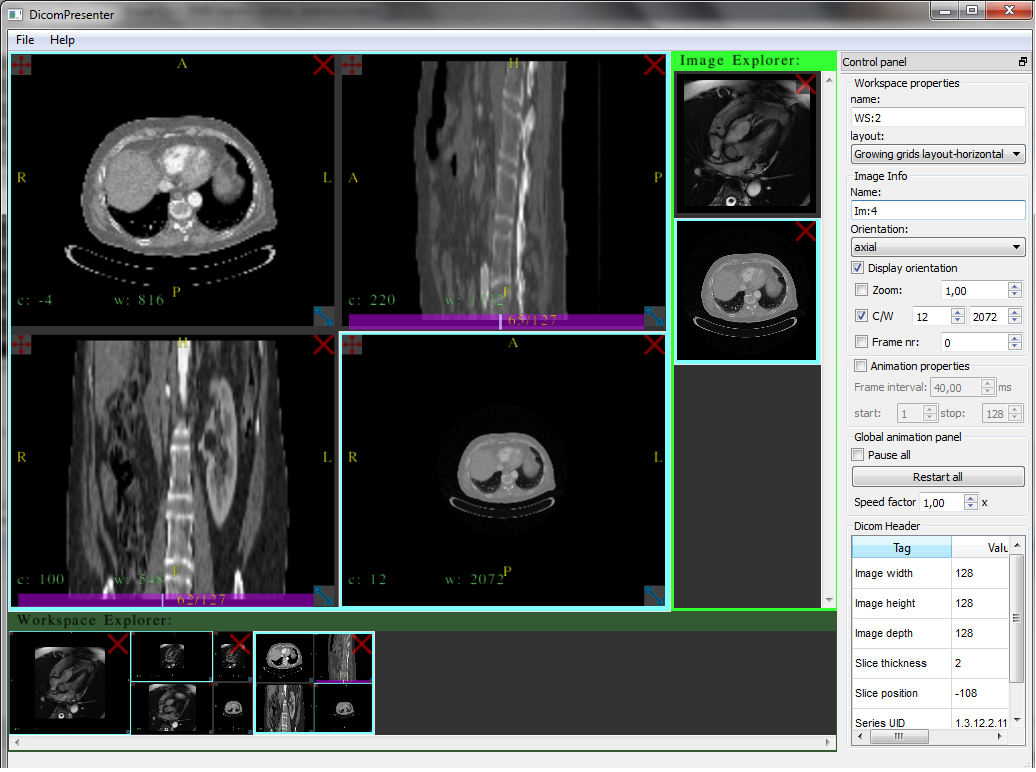
\includegraphics[width=130mm]{Text/IMG/04_GUI_Screenshot.png}
	\end{center}
	\caption{Screenshot of Dicom-Presenter user interface.}
	\label{screenshot}
\end{figure}

\section*{Application requirements}
\addcontentsline{toc}{section}{Application requirements}
The IKEM specialists asked for a typical DICOM images viewer with few more specific features which they missed in freeware programs. A typical DICOM viewer allows you to open .dcm files and display it. .dcm file in this case is a jpeg image equipped with special header including patient's information. There you can see a 2D picture of some part of the patient's body. Some DICOM viewers allow you to open series of .dcm files, which can actually fit into a three-dimensional picture. Less commonly it can be a time animation of organ behaviour in short time period (f.e. one heart beat). DICOM viewers often have some more functions but it is very individual.

There have been two more specific requirements on application functionality by IKEM specialists. They missed certain functions in freeware DICOM applications. The most important function was a possibility to open several images at one time and display them on one screen. The user should be allowed to arrange images on screen to any possible layout he prefers. This functionality allows physicians to see two or more different MRI images on screen so they can easily determine pathological differences among observed organs. It is useful for studying, or teaching.

There have been also requirements that the application should be able to record user's manipulation with images as a video. Then physician can prepare his presentation of images at home and then play the video in front of crowds.

\begin{table}[ht]
	\caption{DICOM viewers.}
	\centering
	\begin{tabular}{cc}
			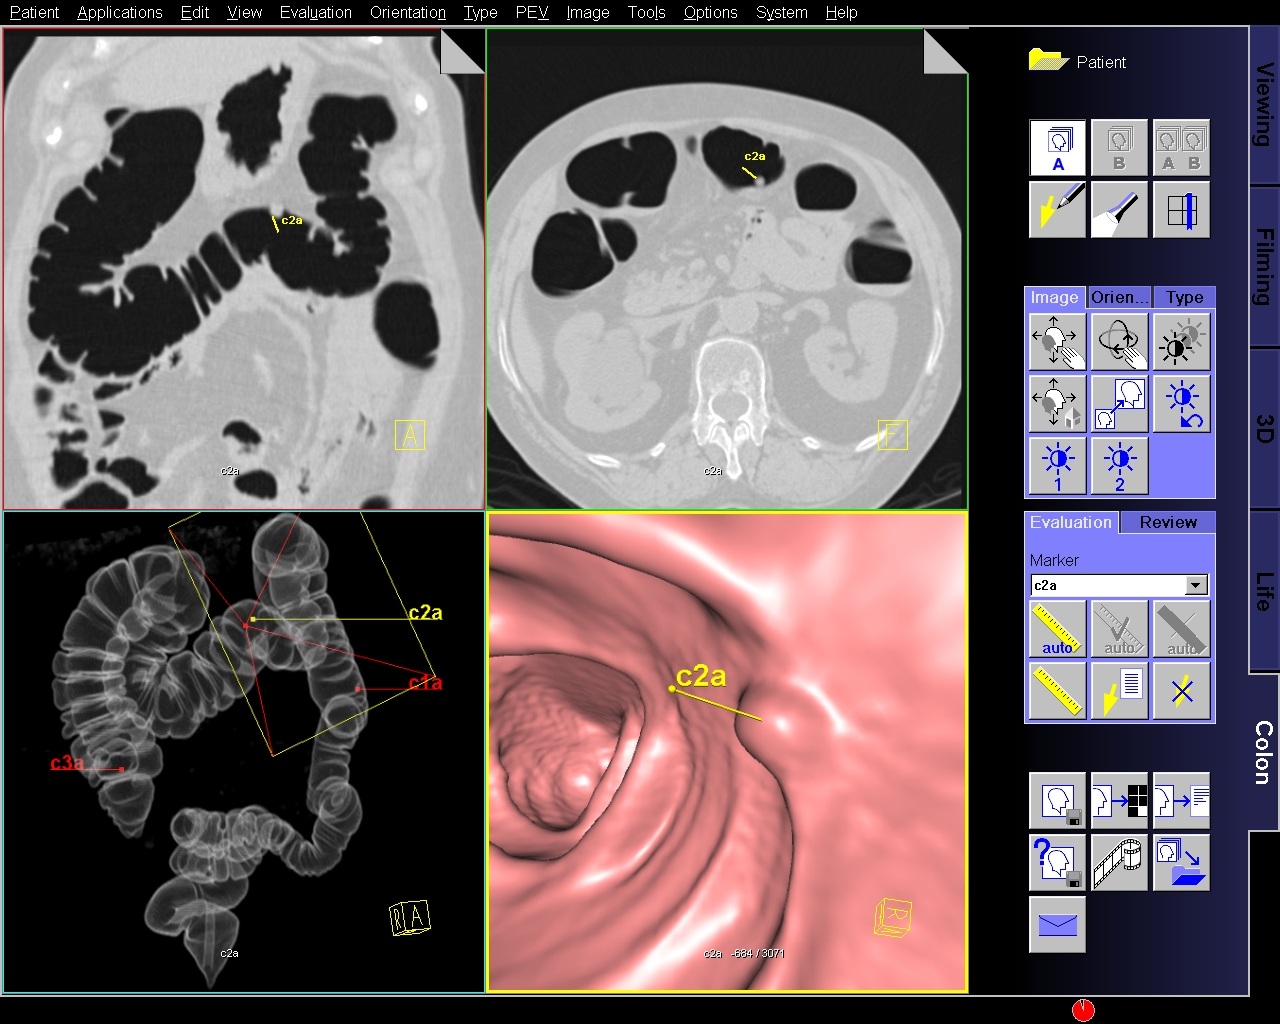
\includegraphics[width=0.5\textwidth,height=0.375\textwidth]{Text/IMG/01_Siemens.jpg}
		&
			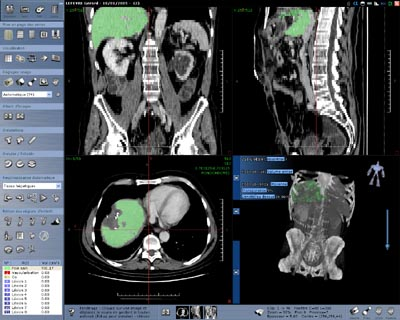
\includegraphics[width=0.5\textwidth,height=0.375\textwidth]{Text/IMG/01_Myrian.jpg}
		\\
			syngo Imaging~\citesec{siemens} & Myrian~\citesec{intrasense}	
		\\
			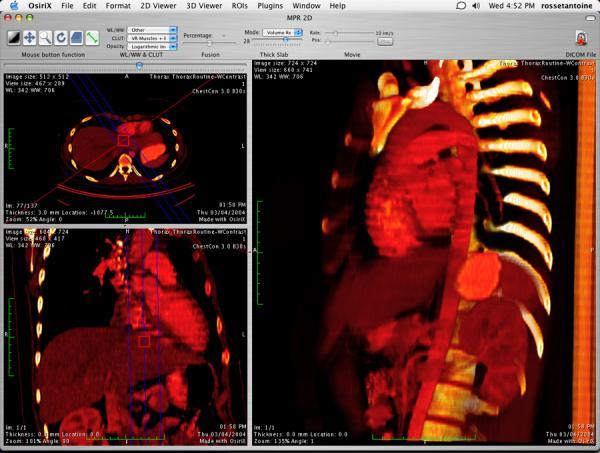
\includegraphics[width=0.5\textwidth,height=0.375\textwidth]{Text/IMG/01_OsiriX.jpg}
		&
			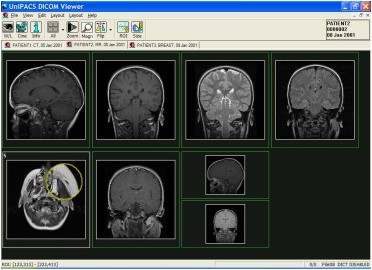
\includegraphics[width=0.5\textwidth,height=0.375\textwidth]{Text/IMG/01_UniPACS.jpg}
		\\
			OsiriX~\citesec{osirix} & UniPACS~\citesec{unipacs}
		\\
		\end{tabular}
\end{table}%

\section*{Application functionality}
\addcontentsline{toc}{section}{Application functionality}

%%%%%%%%%%%%%%%%%%%%%%  DODATKY  %%%%%%%%%%%%%%%%%%%%%%

%\chapter{Dodatky}
%\section{Import kódu}
%\input{Text/07.Import.tex}

%%%%%%%%%%%%%%%%%%%%%%  LITERATURA  %%%%%%%%%%%%%%%%%%%%%%

\nocite{*}				% zobrazuj i necitovane primarni zdroje
\bibliography{Text/Literature}
\nocitesec{*}				% sek. zdroje
\bibliographysec{Text/Zdroje}
\bibliographyurl{Text/Odkazy}


%%%%%%%%%%%%%%%%%%%%%%  PŘÍLOHY %%%%%%%%%%%%%%%%%%%%%%

% \chapter{Přílohy}

% \input{vnitrek_priloha1.tex} % pøíloha 1: vložená z externího souboru
% \input{vnitrek_priloha2.tex} % pøíloha 2: vložená z externího souboru



\end{document}

